\section{Transition Pieces}
\label{sec:transitions}

Often it is necessary to have transitions in the beam pipe which can not be tapered, either due to space constraints or the operational requirements of the device containing the transition. This a common requirement in devices that require some mechanical freedom of movement (i.e. longitudinal or transverse movement is expected), such as bellows, or electrical isolation from the beam pipe, such as kicker magnets. For these devices it is often possible to use a transition piece, that is one or several pieces of conducting material to screen any transition. These may be rigid or moveable as shown in Fig.~\ref{fig:rf_fingers}, often referred to as RF fingers.

\begin{figure}
\begin{center}
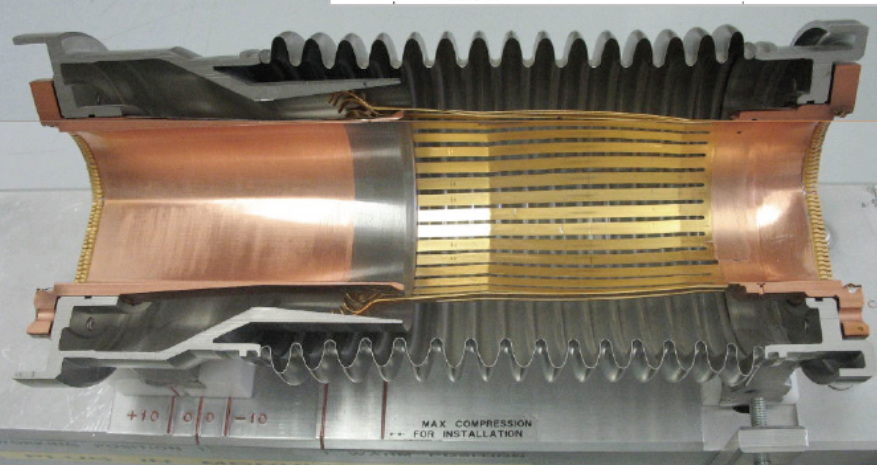
\includegraphics[width=0.45\textwidth]{Beam_Coupling_Impedance_Reduction_Techniques/figures/pimsImage.png}
\label{fig:rf_fingers}
\end{center}
\caption{Example of RF fingers (in this case for the PIMS (Plug In ModuleS) module, placed between cryo-modules in the LHC).}
\end{figure}


This method of impedance reduction is effective for a number of reasons. Firstly it provides a short, good conducting path for the image currents to flow that does not make to the cavity created by the transition visible to the beam, and, in the case of bellows, the image current does not have to follow to long contoured path of the bellows, such as shown in Fig.~\ref{fig:rf_fingers}. This serves to reduce the broadband impedance increase and, by shielding the contours of the bellows, prevents an increase in the imaginary longitudinal impedance due to the increased electrical length of the device. Secondly, by correctly designing the spacing in the transitions, it is possible to minimise field leakage to the surrounding cavities therefore decreasing the visibility of cavity resonances. As an example of a cavity with and without RF fingers and a number of intermediatary steps, see Fig.~\ref{fig:rf_finger_imp}, which illustrates the case of the VMTSA, a vacuum interconnect in the injection region of the LHC \cite{Salvant:VMTSA} containing a double bellow module. It is characterised by a large vacuum chamber (due to the need to contain two circulating beams) with a long set of bellows. The bellows were screened by a long set of RF fingers, which functioned well when good surface contact was maintained between the fingers and the beam pipe. However, when this connection was disrupted (easily created via mechanical stress due to the weak pressure exerted by the afixing spring) the real component of the longitudinal beam coupling impedance increased drastically at around 200MHz, causing further mechanical failure. This highlights the need to correctly consider the mechanical and electromagnetic properties of an impedance reduction system, especially it's possible failure points.


\begin{figure}
\subfigure[]{
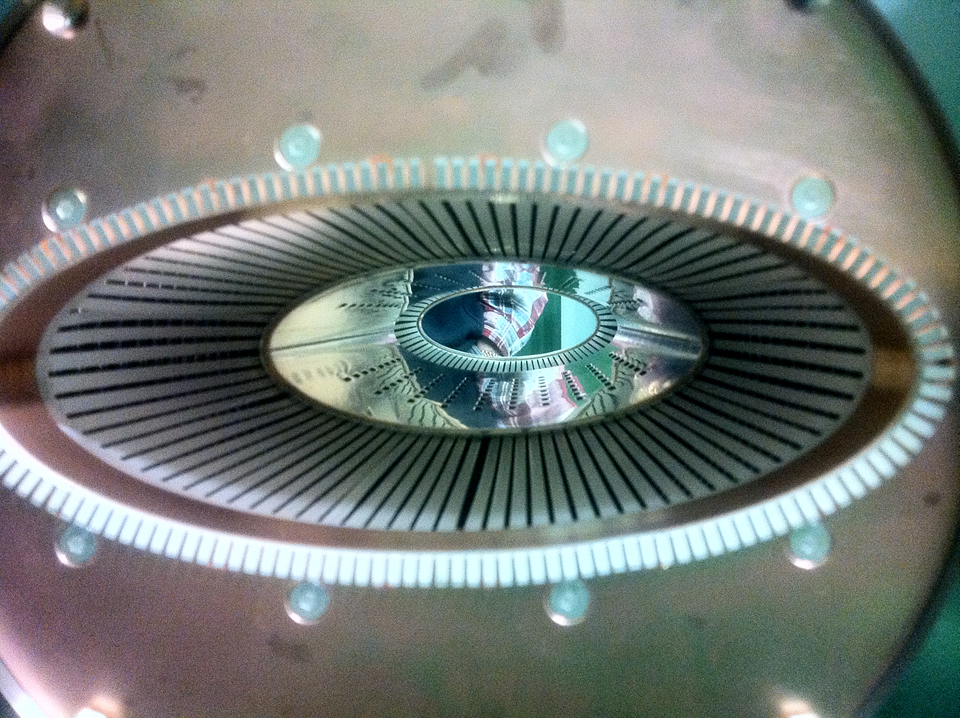
\includegraphics[width=0.45\textwidth]{Beam_Coupling_Impedance_Reduction_Techniques/figures/vmtsa-good-contact.png}
\label{fig:vmtsa_operations}
}
\subfigure[]{
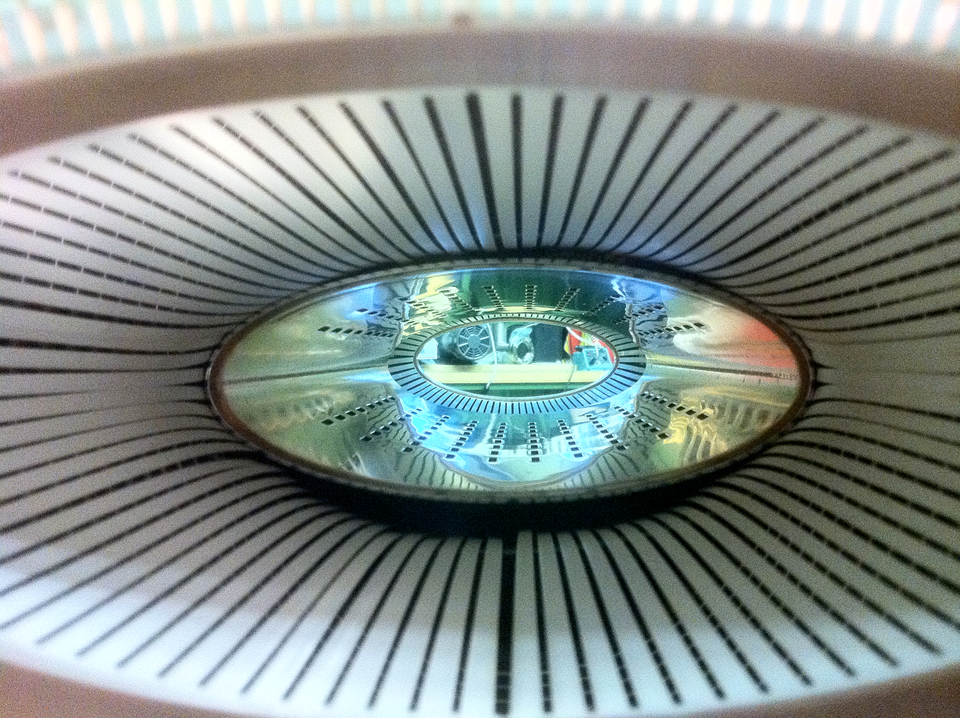
\includegraphics[width=0.45\textwidth]{Beam_Coupling_Impedance_Reduction_Techniques/figures/vmtsa-bad-contact.png}
\label{fig:vmtsa_failure}
}
\begin{center}
\subfigure[]{
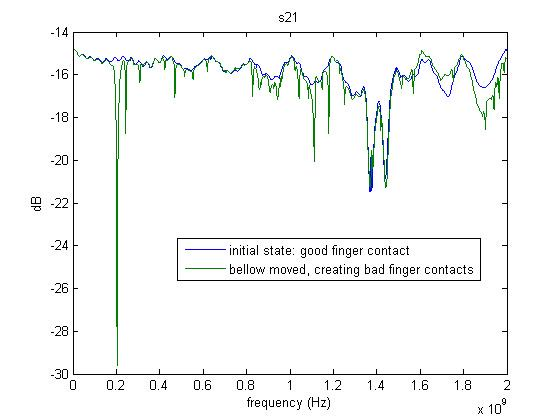
\includegraphics[width=0.7\textwidth]{Beam_Coupling_Impedance_Reduction_Techniques/figures/vmtsa-impedance.png}
\label{fig:vmtsa_impedance}
}
\end{center}
\caption{The layout of the RF fingers in the VMTSA both in \subref{fig:vmtsa_operations} the fully operational configuration and \subref{fig:vmtsa_failure} when some RF fingers lose contact. \subref{fig:vmtsa_impedance} shows the transmission parameter $S_{21}$ for the VMTSA module with and without good electrical contact between the fingers and the beam pipe as acquired by coaxial wire measurements. Photos and measurements courtesy of J.L. Nougaret.}
\label{fig:rf_finger_imp}
\end{figure}